%%-----------------------------------------------------------------------------
%%
%%                                   Sean Mauch
%%                       California Institute of Technology
%%                         @ 1995-2004 No Rights Reserved
%%
%%-----------------------------------------------------------------------------

\flushbottom










%%============================================================================
%%============================================================================
\chapter{Analytic Continuation}


For every complex problem, there is a solution that is simple, neat, and wrong.

\begin{flushright}
  - H. L. Mencken
\end{flushright}






%%==============================================================================
\section{Analytic Continuation}
\index{analytic continuation}



Suppose there is a function, $f_1(z)$ that is analytic in the domain $D_1$ and
another analytic function, $f_2(z)$ that is analytic in the domain $D_2$.
(See Figure~\ref{overlap}.)

\begin{figure}[htb!]
  \begin{center}
    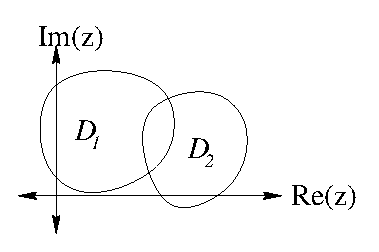
\includegraphics[width=0.25\textwidth]{fcv/continuation/overlap}
  \end{center}
  \caption{Overlapping domains.}
  \label{overlap}
\end{figure}

If the two domains overlap and $f_1(z) = f_2(z)$ in the overlap region 
$D_1 \cap D_2$, then $f_2(z)$ is called an \textit{analytic continuation}
of $f_1(z)$.  This is an appropriate name since $f_2(z)$ continues
the definition of $f_1(z)$ outside of its original domain of definition $D_1$.
We can define a function $f(z)$ that is analytic
in the union of the domains $D_1 \cup D_2$.
On the domain $D_1$ we have $f(z) = f_1(z)$ and $f(z) = f_2(z)$ on $D_2$.
$f_1(z)$ and $f_2(z)$ are called \textit{function elements}.
\index{function elements}
There is an analytic continuation even if the two domains only share
an arc and not a two dimensional region.



With more overlapping domains $D_3, D_4, \ldots$ we could perhaps extend 
$f_1(z)$ to more of the complex plane.  Sometimes it is impossible to
extend a function beyond the boundary of a domain.  This is known
as a \textit{natural boundary}.
\index{natural boundary}
%% CONTINUE: do an example of a natural boundary.
If a function $f_1(z)$ is analytically continued to a domain $D_n$ along two
different paths, (See Figure~\ref{twopaths}.), then the two analytic 
continuations are identical as long as the paths do not enclose a branch
point of the function.  This is the \textit{uniqueness theorem of 
  analytic continuation}.

\begin{figure}[htb!]
  \begin{center}
    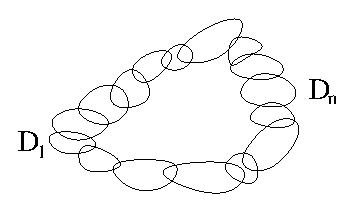
\includegraphics[width=0.25\textwidth]{fcv/continuation/twopaths}
  \end{center}
  \caption{Two paths of analytic continuation.}
  \label{twopaths}
\end{figure}




Consider an analytic function $f(z)$ defined in the domain $D$.  Suppose
that $f(z) = 0$ on the arc $AB$, (see Figure~\ref{zeroarc}.)  Then
$f(z) = 0$ in all of $D$.

\begin{figure}[htb!]
  \begin{center}
    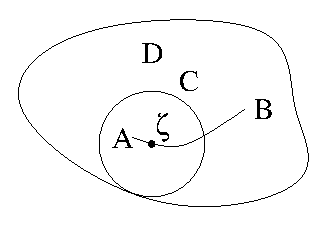
\includegraphics[width=0.2\textwidth]{fcv/continuation/zeroarc}
  \end{center}
  \caption{The domain containing the arc along which the function
    vanishes.}
  \label{zeroarc}
\end{figure}

Consider a point $\zeta$ on $AB$.  The Taylor series expansion of $f(z)$
about the point $z=\zeta$ converges in a circle $C$ at least up to the boundary
of $D$.  The derivative of $f(z)$ at the point $z = \zeta$ is
\[
f'(\zeta) 
= \lim_{\Delta z \to 0} \frac{f(\zeta + \Delta z) - f(\zeta)}{\Delta z}
\]
If $\Delta z$ is in the direction of the arc, then $f'(\zeta)$
vanishes as well as all higher derivatives, $f'(\zeta) = f''(\zeta) = 
f'''(\zeta) = \cdots = 0$.  Thus we see that $f(z) = 0$ inside $C$.  
By taking Taylor series expansions about points on $AB$ or inside of $C$ we
see that $f(z) = 0$ in $D$.





\begin{Result}
  \label{continuation1}
  Let $f_1(z)$ and $f_2(z)$ be analytic functions defined in $D$.  If 
  $f_1(z) = f_2(z)$ for the points in a region or on an arc in $D$, then
  $f_1(z) = f_2(z)$ for all points in $D$.  
\end{Result}


To prove Result~\ref{continuation1}, we define the 
analytic function $g(z) = f_1(z) - f_2(z)$.  Since $g(z)$ vanishes
in the region or on the arc, then $g(z) = 0$ and hence $f_1(z) = f_2(z)$
for all points in $D$.





\begin{Result}
  \label{continuation2}
  Consider analytic functions $f_1(z)$ and $f_2(z)$ defined on the 
  domains $D_1$ and $D_2$, respectively.  Suppose that $D_1 \cap D_2$ is
  a region or an arc and that $f_1(z) = f_2(z)$ for all $z \in D_1 \cap D_2$.
  (See Figure~\ref{interra}.) Then the function
  \[
  f(z) = 
  \begin{cases}
    f_1(z) &\mathrm{for}\ z \in D_1, \\
    f_2(z) &\mathrm{for}\ z \in D_2,
  \end{cases}
  \]
  is analytic in $D_1 \cup D_2$.
\end{Result}


\begin{figure}[htb!]
  \begin{center}
    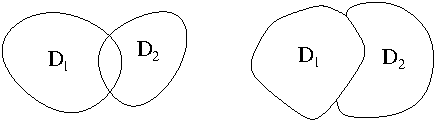
\includegraphics[width=0.4\textwidth]{fcv/continuation/interra}
  \end{center}
  \caption{Domains that intersect in a region or an arc.}
  \label{interra}
\end{figure}

Result~\ref{continuation2} follows directly from Result~\ref{continuation1}.

%% CONTINUE: analytically continue the Gamma function.



%%==============================================================================
\section{Analytic Continuation of Sums}



\begin{Example}
  Consider the function
  \[
  f_1(z) = \sum_{n = 0}^\infty z^n.
  \]
  The sum converges uniformly for $D_1 = |z| \leq r < 1$.
  Since the derivative also
  converges in this domain, the function is analytic there.

  \begin{figure}[htb!]
    \begin{center}
      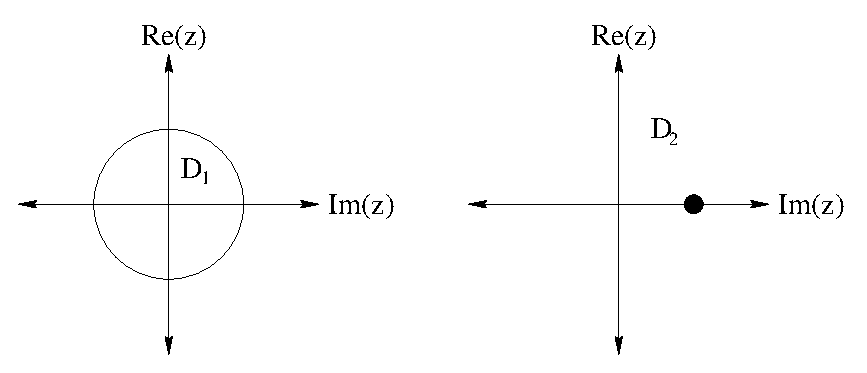
\includegraphics[width=0.6\textwidth]{fcv/continuation/ooomz}
    \end{center}
    \caption{The domain of convergence.}
    \label{ooomz}
  \end{figure}

  Now consider the function
  \[
  f_2(z) =  \frac{1}{1-z}.
  \]
  This function is analytic everywhere except the point $z = 1$.  On the
  domain $D_1$,
  \[
  f_2(z) = \frac{1}{1-z} = \sum_{n = 0}^\infty z^n = f_1(z)
  \]

  Analytic continuation tells us that there is a function that is analytic
  on the union of the two domains.  Here, the domain is the entire $z$ plane
  except the point $z = 1$ and the function is
  \[ f(z) = \frac{1}{1-z}. \]
  $\frac{1}{1-z}$ is said to be an analytic continuation of
  $\sum_{n = 0}^\infty z^n$.
\end{Example}









%%==============================================================================
\section{Analytic Functions Defined in Terms of Real Variables}







\begin{Result}
  \label{ancontuvtz}%%HERE
  An analytic function, $u(x,y) + \imath v(x,y)$ can be written in terms of a 
  function of a complex variable, $f(z) = u(x,y) + \imath v(x,y)$.
\end{Result}

Result~\ref{ancontuvtz} is proved in Exercise~\ref{prob_real2complex}.










\begin{Example}
  \begin{align*}
    f(z) &= \cosh y \sin x  \left( x \e^x \cos y - y \e^x \sin y \right)
    - \cos x \sinh y \left( y \e^x \cos y + x \e^x \sin y \right) 
    \\
    &\qquad + \imath \big[ \cosh y \sin x \left( y \e^x \cos y 
      + x \e^x \sin y \right)
    + \cos x \sinh y \left( x \e^x \cos y - y \e^x \sin y \right) \big]
  \end{align*}
  is an analytic function.
  Express $f(z)$ in terms of $z$.

  \vspace{0.1in}

  On the real line, $y = 0$, $f(z)$ is
  \[
  f(z = x) = x \e^x \sin x
  \]
  (Recall that $\cos(0) = \cosh(0) = 1$ and $\sin(0) = \sinh(0) = 0$.)

  The analytic continuation of $f(z)$ into the complex plane is
  \[
  \boxed{ f(z) = z \e^z \sin z. }
  \]

  Alternatively, for $x = 0$ we have
  \[
  f(z = \imath y) = y \sinh y (\cos y - \imath \sin y).
  \]
  The analytic continuation from the imaginary axis to the complex plane is
  \begin{align*}
    f(z)    
    &= -\imath z \sinh(-\imath z)  (\cos(-\imath z) - \imath \sin(-\imath z)) 
    \\
    &= \imath z \sinh(\imath z)  (\cos(\imath z) + \imath \sin(\imath z)) 
    \\
    &= z \sin z \e^z.
  \end{align*}
\end{Example}








\begin{Example}
  Consider $u = \e^{-x} (x \sin y - y \cos y)$.
  Find $v$ such that $f(z) = u + \imath v$ is analytic.

  From the Cauchy-Riemann equations,
  \begin{gather*}
    \frac{\partial v}{\partial y} = \frac{\partial u}{\partial x} =
    \e^{-x} \sin y - x \e^{-x} \sin y + y \e^{-x} \cos y
    \\
    \frac{\partial v}{\partial x} = -\frac{\partial u}{\partial y} =
    \e^{-x} \cos y - x \e^{-x} \cos y - y \e^{-x} \sin y
  \end{gather*}
  Integrate the first equation with respect to $y$.
  \begin{align*}
    v &= -\e^{-x} \cos y + x \e^{-x} \cos y + \e^{-x} (y \sin y + \cos y) + F(x) 
    \\
    &= y \e^{-x} \sin y + x \e^{-x} \cos y + F(x)
  \end{align*}
  $F(x)$ is an arbitrary function of $x$.
  Substitute this expression for $v$ into the equation for
  $\partial v/ \partial x$.
  \[
  -y \e^{-x} \sin y - x \e^{-x} \cos y + \e^{-x} \cos y + F'(x) =
  -y \e^{-x} \sin y - x \e^{-x} \cos y + \e^{-x} \cos y
  \]
  Thus $F'(x) = 0$ and $F(x) = c$.
  \[
  v = \e^{-x} (y \sin y + x \cos y) + c
  \]
\end{Example}









\begin{Example}
  Find $f(z)$ in the previous example.  (Up to the additive constant.)

  \paragraph{Method 1}
  \begin{align*}
    f(z) &= u + \imath v 
    \\
    &= \e^{-x} (x \sin y - y \cos y) + \imath \e^{-x} (y \sin y + x \cos y) 
    \\
    &= \e^{-x} \left\{ x \left( \frac{\e^{\imath y} - \e^{-\imath y}}{\imath 2} \right)
      - y \left( \frac{\e^{\imath y} + \e^{-\imath y}}{2} \right) \right\} +
    \imath \e^{-x} \left\{ y \left(\frac{\e^{\imath y}-\e^{-\imath y}}{\imath 2} \right) +
      x \left( \frac{\e^{\imath y} + \e^{-\imath y}}{2} \right) \right\} 
    \\
    &= \imath (x + \imath y) \e^{-(x + \imath y)} 
    \\
    &= \imath z \e^{-z}
  \end{align*}

  \paragraph{Method 2}
  $f(z) = f(x + \imath y) = u(x,y) + \imath v(x,y)$ is an analytic function.

  On the real axis, $y = 0$, $f(z)$ is
  \begin{align*}
    f(z = x) &= u(x,0) + \imath v(x,0) 
    \\
    &= \e^{-x} (x \sin 0 - 0 \cos 0) + \imath \e^{-x} (0 \sin 0 + x \cos 0) 
    \\
    &= \imath x \e^{-x}
  \end{align*}
  Suppose there is an analytic continuation of $f(z)$ into the complex plane.
  If such a continuation, $f(z)$, exists, then it must be equal to $f(z = x)$
  on the real axis
  An obvious choice for the analytic continuation is
  \[
  f(z) = u(z, 0) + \imath v(z, 0)
  \]
  since this is clearly equal to $u(x, 0) + \imath v(x, 0)$ when $z$ is real.
  Thus we obtain
  \[  
  f(z) = \imath z \e^{-z} 
  \]
\end{Example}




\begin{Example}
  Consider $f(z) = u(x, y) + \imath v(x, y)$.
  Show that
  $f'(z) = u_x(z,0) - \imath u_y(z,0)$.
  \begin{align*}
    f'(z) &= u_x + \imath v_x 
    \\
    &= u_x - \imath u_y
  \end{align*}
  $f'(z)$ is an analytic function.  On the real axis, $z = x$, $f'(z)$ is
  \[
  f'(z = x) = u_x(x,0) - \imath u_y(x,0)
  \]
  Now $f'(z = x)$ is defined on the real line.  An analytic continuation of
  $f'(z = x)$ into the complex plane is
  \[
  \boxed{ 
    f'(z) = u_x(z, 0) - \imath u_y(z, 0). 
    }
  \]
\end{Example}









\begin{Example}
  Again consider the problem of finding $f(z)$ given that
  $u(x, y) = \e^{-x} (x \sin y - y \cos y )$.
  Now we can use the result of the previous example to do this problem.
  \begin{align*}
    u_x(x,y) &= \frac{\partial u}{\partial x} =
    \e^{-x} \sin y - x \e^{-x} \sin y + y \e^{-x} \cos y 
    \\
    u_y(x,y) &= \frac{\partial u}{\partial y} = x \e^{-x} \cos y + y \e^{-x} \sin y 
    - \e^{-x} \cos y
  \end{align*}
  \begin{align*}
    f'(z) &= u_x(z,0) - \imath u_y(z,0) 
    \\
    &= 0 - \imath \left( z \e^{-z} - \e^{-z} \right) 
    \\
    &= \imath \left( -z \e^{-z} + \e^{-z} \right)
  \end{align*}
  Integration yields the result
  \[
  \boxed{ 
    f(z) = \imath z\e^{-z} + c 
    }
  \]
\end{Example}







\begin{Example}
  Find $f(z)$ given that
  \begin{align*}
    u(x,y)  &= \cos x \cosh^2 y \sin x + \cos x \sin x \sinh^2 y 
    \\
    v(x,y)  &= \cos^2 x \cosh y \sinh y - \cosh y \sin^2 x \sinh y
  \end{align*}

  \vspace{0.1in}
  $f(z) = u(x,y) + \imath v(x,y)$ is an analytic function.  On the real line,
  $f(z)$ is
  \begin{align*}
    f(z = x)  &= u(x,0) + \imath v(x,0) 
    \\
    &= \cos x \cosh^2 0 \sin x + \cos x \sin x \sinh^2 0
    + \imath \left( \cos^2 x \cosh 0 \sinh 0 - \cosh 0 \sin^2 x \sinh 0 \right) 
    \\
    &= \cos x \sin x
  \end{align*}
  Now we know the definition of $f(z)$ on the real line.  We would like to find
  an analytic continuation of $f(z)$ into the complex plane.  An obvious
  choice for $f(z)$ is
  \[
  f(z) = \cos z \sin z
  \]
  Using trig identities we can write this as
  \[
  \boxed{ 
    f(z) = \frac{\sin(2 z)}{2}. 
    }
  \]
\end{Example}





\begin{Example}
  Find $f(z)$ given only that
  \[
  u(x,y)  = \cos x \cosh^2 y \sin x + \cos x \sin x \sinh^2 y.
  \]


  Recall that
  \begin{align*}
    f'(z) &= u_x + \imath v_x 
    \\
    &= u_x - \imath u_y
  \end{align*}
  Differentiating $u(x, y)$,
  \begin{align*}
    u_x &= \cos^2 x \cosh^2 y - \cosh^2 y \sin^2 x + \cos^2 x \sinh^2 y -
    \sin^2 x \sinh^2 y \\
    u_y &= 4 \cos x \cosh y \sin x \sinh y
  \end{align*}

  $f'(z)$ is an analytic function.  On the real axis, $f'(z)$ is
  \[
  f'(z = x) = \cos^2 x - \sin^2 x
  \]
  Using trig identities we can write this as
  \[
  f'(z = x) = \cos(2 x)
  \]
  Now we find an analytic continuation of $f'(z = x)$ into the complex plane.
  \[
  f'(z) = \cos(2 z)
  \]
  Integration yields the result
  \[
  \boxed{ 
    f(z) = \frac{\sin(2 z)}{2} + c 
    }
  \]
\end{Example}







\subsection{Polar Coordinates}



\begin{Example}
  Is
  \[
  u(r,\theta) = r ( \log r \cos \theta - \theta \sin \theta )
  \]
  the real part of an analytic function?


  The Laplacian in polar coordinates is
  \[
  \Delta \phi = \frac{1}{r} \frac{\partial}{\partial r} \left( r \frac{\partial \phi}{\partial r} \right)
  + \frac{1}{r^2} \frac{\partial^2 \phi}{\partial \theta^2}.
  \]
  We calculate the partial derivatives of $u$.
  \begin{align*}
    \frac{\partial u}{\partial r} &= \cos \theta + \log r \cos \theta - \theta \sin \theta 
    \\
    r \frac{\partial u}{\partial r} &= r \cos \theta + r \log r \cos \theta
    - r \theta \sin \theta 
    \\
    \frac{\partial}{\partial r} \left( r \frac{\partial u}{\partial r} \right)
    &= 2 \cos \theta + \log r \cos \theta - \theta \sin \theta 
    \\
    \frac{1}{r} \frac{\partial}{\partial r} \left( r \frac{\partial u}{\partial r} \right)
    &= \frac{1}{r} \left( 2  \cos \theta +  \log r \cos \theta -  \theta \sin \theta \right) 
    \\
    \frac{\partial u}{\partial \theta} &= -r \left( \theta \cos \theta + \sin \theta + \log r \sin \theta \right) 
    \\
    \frac{\partial^2 u}{\partial \theta^2} &= r \left( - 2 \cos \theta - \log r \cos \theta 
      + \theta \sin \theta \right) 
    \\
    \frac{1}{r^2} \frac{\partial^2 u}{\partial \theta^2} &= \frac{1}{r} 
    \left( - 2 \cos \theta - \log r \cos \theta + \theta \sin \theta \right)
  \end{align*}
  From the above we see that
  \[
  \Delta u = \frac{1}{r} \frac{\partial}{\partial r} \left( r \frac{\partial u}{\partial r} \right)
  + \frac{1}{r^2} \frac{\partial^2 u}{\partial \theta^2} = 0.
  \]
  Therefore $u$ is harmonic and is the real part of some analytic function.
\end{Example}








\begin{Example}
  Find an analytic function $f(z)$ whose real part is
  \[
  u(r,\theta) =  r \left( \log r \cos \theta - \theta \sin \theta \right).
  \]

  Let $f(z) = u(r,\theta) + \imath v(r,\theta)$.
  The Cauchy-Riemann equations are
  \[
  u_r = \frac{v_\theta}{r}, \qquad u_\theta = -r v_r.
  \]
  Using the partial derivatives in the above example, we obtain two partial
  differential equations for $v(r, \theta)$.
  \begin{align*}
    v_r &= -\frac{u_\theta}{r} = \theta \cos \theta + \sin \theta + \log r \sin \theta  
    \\
    v_\theta &= r u_r = r \left( \cos \theta + \log r \cos \theta - \theta \sin \theta \right)
  \end{align*}

  Integrating the equation for $v_\theta$ yields
  \[
  v = r \left( \theta \cos \theta + \log r \sin \theta \right) + F(r)
  \]
  where $F(r)$ is a constant of integration.

  Substituting our expression for $v$ into the equation for $v_r$ yields
  \begin{gather*}
    \theta \cos \theta + \log r \sin \theta + \sin \theta + F'(r) =
    \theta \cos \theta + \sin \theta + \log r \sin \theta 
    \\
    F'(r) = 0 \\
    F(r) = \mathrm{const}
  \end{gather*}

  Thus we see that
  \begin{align*}
    f(z)
    &= u + \imath v 
    \\
    &= r \left( \log r \cos \theta - \theta \sin \theta \right)
    + \imath r \left( \theta \cos \theta + \log r \sin \theta \right)
    + \mathrm{const}
  \end{align*}

  $f(z)$ is an analytic function. On the line $\theta = 0$, $f(z)$ is
  \begin{align*}
    f(z = r) &= r ( \log r ) + \imath r ( 0 ) + \mathrm{const} 
    \\
    &= r \log r + \mathrm{const}
  \end{align*}
  The analytic continuation into the complex plane is
  \[
  \boxed{ 
    f(z) = z \log z + \mathrm{const} 
    }
  \]
\end{Example}







\begin{Example}
  Find the formula in polar coordinates that is analogous to
  \[
  f'(z) = u_x(z, 0) - \imath u_y(z,0).
  \]

  We know that
  \[
  \frac{\dd f}{\dd z} = \e^{-\imath \theta} \frac{\partial f}{\partial r}.
  \]
  If $f(z) = u(r,\theta) + \imath v(r,\theta)$ then
  \[
  \frac{\dd f}{\dd z} = \e^{-\imath \theta} \left( u_r + \imath v_r \right)
  \]
  From the Cauchy-Riemann equations, we have $v_r = -u_\theta / r$.
  \[
  \frac{\dd f}{\dd z} = \e^{-\imath \theta} \left( u_r - \imath \frac{ u_\theta}{r} \right)
  \]

  $f'(z)$ is an analytic function.  On the line $\theta = 0$, $f(z)$ is
  \[
  f'(z = r) = u_r(r,0) - \imath \frac{u_\theta(r,0)}{r}
  \]
  The analytic continuation of $f'(z)$ into the complex plane is
  \[
  \boxed{ 
    f'(z) = u_r(z, 0) - \frac{\imath}{r} u_\theta(z,0). 
    }
  \]
\end{Example}





\begin{Example}
  Find an analytic function $f(z)$ whose real part is
  \[
  u(r,\theta) =  r \left( \log r \cos \theta - \theta \sin \theta \right).
  \]

  \begin{align*}
    u_r(r, \theta) &= \left( \log r \cos \theta - \theta \sin \theta \right) + \cos \theta 
    \\
    u_\theta(r,\theta) &= r \left( -\log r \sin \theta - \sin \theta - \theta \cos \theta \right)
  \end{align*}
  \begin{align*}
    f'(z)
    &= u_r(z,0) - \frac{\imath}{r} u_\theta(z,0) 
    \\
    &= \log z + 1
  \end{align*}
  Integrating $f'(z)$ yields
  \[
  \boxed{ 
    f(z) = z \log z + \imath c. 
    }
  \]
\end{Example}






%%-----------------------------------------------------------------------------
\subsection{Analytic Functions Defined in Terms of Their Real or Imaginary
  Parts}




Consider an analytic function: $f(z) = u(x,y) + \imath v(x,y)$.
We differentiate this expression.
\[
f'(z) = u_x(x,y) + \imath v_x(x,y)
\]
We apply the Cauchy-Riemann equation $v_x = - u_y$.
\begin{equation}
  \label{eqn_fpz_uxmiuy}
  f'(z) = u_x(x,y) - \imath u_y(x,y).
\end{equation}
Now consider the function of a complex variable, $g(\zeta)$:
\[
g(\zeta) = u_x(x, \zeta) - \imath u_y(x, \zeta)
= u_x(x, \xi + \imath \psi ) - \imath u_y(x, \xi + \imath \psi ).
\]
This function is analytic where $f(\zeta)$ is analytic.  To show this we 
first verify that the derivatives in the $\xi$ and $\psi$ directions
are equal.
\begin{gather*}
  \frac{\partial}{\partial \xi} g(\zeta) 
  = u_{x y}(x, \xi + \imath \psi) - \imath u_{y y}(x, \xi + \imath \psi) 
  \\
  -\imath \frac{\partial}{\partial \psi} g(\zeta) 
  = -\imath \left( \imath u_{x y}(x, \xi + \imath \psi) + u_{y y}(x, \xi + \imath \psi) \right) 
  = u_{x y}(x, \xi + \imath \psi) - \imath u_{y y}(x, \xi + \imath \psi)
\end{gather*}
Since these partial derivatives are equal and continuous, $g(\zeta)$ is 
analytic.  We evaluate the function $g(\zeta)$ at $\zeta = -\imath x$.
(Substitute $y = - \imath x$ into Equation~\ref{eqn_fpz_uxmiuy}.)
\[
f'(2 x) = u_x(x,-\imath x) - \imath u_y(x,-\imath x)
\]
We make a change of variables to solve for $f'(x)$.
\[
f'(x) = u_x \left( \frac{x}{2}, -\imath \frac{x}{2} \right) 
- \imath u_y\left( \frac{x}{2}, -\imath \frac{x}{2} \right).
\]
If the expression is non-singular, then
this defines the analytic function, $f'(z)$, on the real axis.  The analytic
continuation to the complex plane is
\[
f'(z) = u_x \left( \frac{z}{2}, -\imath \frac{z}{2} \right) 
- \imath u_y \left( \frac{z}{2}, -\imath \frac{z}{2} \right).
\]
Note that 
$\frac{\dd}{\dd z} 2 u(z/2, -\imath z/2) = u_x(z/2, -\imath z/2) -\imath u_y(z/2, -\imath z/2)$.
We integrate the equation to obtain:
\[
f(z) = 2 u \left( \frac{z}{2}, -\imath \frac{z}{2} \right) + c.
\]
We know that the real part of an analytic function determines that 
function to within an additive constant.
Assuming that the above expression is non-singular, we have found a formula
for writing an analytic function in terms of its real part.  
With the same method, we can find how to write an analytic function in terms 
of its imaginary part, $v$.

We can also derive formulas if $u$ and $v$ are expressed in polar coordinates:
\[
f(z) = u(r, \theta) + \imath v(r, \theta).
\]


\begin{Result}
  If $f(z) = u(x,y) + \imath v(x,y)$ is analytic 
  and the expressions are non-singular, then 
  \begin{align}
    \label{eqn_fz_2u_xy}
    f(z) &= 2 u \left( \frac{z}{2}, -\imath \frac{z}{2} \right) 
    + \mathrm{const} 
    \\
    f(z) &= \imath 2 v \left( \frac{z}{2}, -\imath \frac{z}{2} \right) 
    + \mathrm{const}.
  \end{align}
  %%
  If $f(z) = u(r,\theta) + \imath v(r,\theta)$ is analytic 
  and the expressions are non-singular, then 
  \begin{align}
    \label{eqn_fz_2u_rt}
    f(z) &= 2 u \left( z^{1/2}, - \frac{\imath}{2} \log z \right) + \mathrm{const} 
    \\
    f(z) &= \imath 2 v \left( z^{1/2}, - \frac{\imath}{2} \log z \right) + \mathrm{const}.
  \end{align}
\end{Result}






\begin{Example}
  Consider the problem of finding $f(z)$ given that
  $u(x, y) = \e^{-x} (x \sin y - y \cos y )$.

  \begin{align*}
    f(z)    
    &= 2 u \left( \frac{z}{2}, -\imath \frac{z}{2} \right) \\
    &= 2 \e^{-z/2} \left( \frac{z}{2} \sin \left( - \imath \frac{z}{2} \right)
      + \imath \frac{z}{2} \cos \left( -\imath \frac{z}{2} \right) \right) + c 
    \\
    &= \imath z \e^{-z/2} \left( \imath \sin \left( \imath \frac{z}{2} \right)
      + \cos \left( -\imath \frac{z}{2} \right) \right) + c 
    \\
    &= \imath z \e^{-z/2} \left( \e^{-z/2} \right) + c 
    \\
    &= \imath z \e^{-z} + c 
  \end{align*}
\end{Example}









\begin{Example}
  Consider
  \[
  \Log z = \frac{1}{2} \Log \left( x^2 + y^2 \right) + \imath \Arctan(x, y).
  \]
  We try to construct the analytic function from its real part using
  Equation~\ref{eqn_fz_2u_xy}. 
  \begin{align*}
    f(z)
    &= 2 u \left( \frac{z}{2}, -\imath \frac{z}{2} \right) + c
    \\
    &= 2 \frac{1}{2} \Log \left( \left( \frac{z}{2} \right)^2
      + \left( -\imath \frac{z}{2} \right)^2 \right) + c
    \\
    &= \Log(0) + c
  \end{align*}
  We obtain a singular expression, so the method fails.
\end{Example}






\begin{Example}
  Again consider the logarithm, this time written in terms of polar 
  coordinates.
  \[
  \Log z = \Log r + \imath \theta
  \]
  We try to construct the analytic function from its real part using
  Equation~\ref{eqn_fz_2u_rt}. 
  \begin{align*}
    f(z)
    &= 2 u \left( z^{1/2}, -\imath \frac{\imath}{2} \log z \right) + c 
    \\
    &= 2 \Log \left( z^{1/2} \right) + c 
    \\
    &= \Log z + c
  \end{align*}
  With this method we recover the analytic function.
\end{Example}







\raggedbottom
%%=============================================================================
\exercises{
\pagebreak
\flushbottom
\section{Exercises}








%%11111111111111111111111111111111111111111111111111111111111111111111111111111
\begin{Exercise}
  Consider two functions, $f(x,y)$ and $g(x,y)$.  They are said to be 
  functionally dependent if there is a an $h(g)$ such that
  \[
  f(x,y) = h(g(x,y)).
  \]
  $f$ and $g$ will be functionally dependent if and only if their Jacobian 
  vanishes.

  If $f$ and $g$ are functionally dependent, then the derivatives of $f$ are
  \begin{align*}
    f_x &= h'(g) g_x 
    \\
    f_y &= h'(g) g_y.
  \end{align*}
  Thus we have 
  \[
  \frac{\partial(f,g)}{\partial(x,y)} 
  = \begin{vmatrix}
    f_x     &       f_y 
    \\
    g_x     &       g_y
  \end{vmatrix}
  = f_x g_y - f_y g_x
  = h'(g) g_x g_y - h'(g) g_y g_x
  = 0.
  \]
  If the Jacobian of $f$ and $g$ vanishes, then
  \[
  f_x g_y - f_y g_x = 0.
  \]
%%%% CONTINUE
%%%% Prove this.
  This is a first order partial differential equation for $f$ that has the 
  general solution
  \[
  f(x,y) = h(g(x,y)).
  \]

  Prove that an analytic function $u(x,y) + \imath v(x,y)$ can be written in terms
  of a function of a complex variable, $f(z) = u(x,y) + \imath v(x,y)$.
\end{Exercise}






%%
\begin{Exercise}
  Which of the following functions are the real part of an analytic function?
  For those that are, find the harmonic conjugate, $v(x,y)$, and find the
  analytic function $f(z) = u(x,y) + \imath v(x,y)$ as a function of $z$.
  \begin{enumerate}
  \item $x^3 - 3 x y^2 - 2 x y + y$
  \item $\e^x \sinh y$
  \item $\e^x \left( \sin x \cos y \cosh y - \cos x \sin y \sinh y \right)$
  \end{enumerate}
\end{Exercise}








%% f(z) = 2 u \left( z^{1/2}, - \frac{\imath}{2} \log z \right) + \mathrm{const}.
\begin{Exercise}
  For an analytic function, $f(z) = u(r, \theta) + \imath v(r, \theta)$ prove
  that under suitable restrictions:
  \[
  f(z) = 2 u \left( z^{1/2}, - \frac{\imath}{2} \log z \right) + \mathrm{const}.
  \]
\end{Exercise}






\raggedbottom
}
%%=============================================================================
\hints{
\pagebreak
\flushbottom
\section{Hints}



%%11111111111111111111111111111111111111111111111111111111111111111111111111111
\begin{Hint}
  Show that $u(x,y) + \imath v(x,y)$ is functionally dependent on $x + \imath y$ so that
  you can write $f(z) = f(x + \imath y) = u(x,y) + \imath v(x,y)$.
\end{Hint}





%%
\begin{Hint}
  %% CONTINUE
\end{Hint}




%% f(z) = 2 u \left( z^{1/2}, - \frac{\imath}{2} \log z \right) + \mathrm{const}.
\begin{Hint}
  Check out the derivation of Equation~\ref{eqn_fz_2u_xy}.
\end{Hint}









\raggedbottom
}
%%=============================================================================
\solutions{
\pagebreak
\flushbottom
\section{Solutions}






%%11111111111111111111111111111111111111111111111111111111111111111111111111111
\begin{Solution}
  \label{prob_real2complex}
  $u(x,y) + \imath v(x,y)$ is functionally dependent on $z = x + \imath y$ 
  if and only if
  \[
  \frac{\partial(u + \imath v,x + \imath y)}{\partial(x,y)} = 0.
  \]
  \begin{align*}
    \frac{\partial(u + \imath v,x + \imath y)}{\partial(x,y)} 
    &= \begin{vmatrix}
      u_x + \imath v_x     &       u_y + \imath v_y 
      \\
      1               &       \imath
    \end{vmatrix} \\
    &= -v_x - u_y + \imath \left( u_x - v_y \right) 
    \\
    \intertext{Since $u$ and $v$ satisfy the Cauchy-Riemann equations, this 
      vanishes.}
    &= 0
  \end{align*}
  Thus we see that $u(x,y) + \imath v(x,y)$ is functionally dependent on 
  $x + \imath y$ so we can write
  \[
  f(z) = f(x + \imath y) = u(x,y) + \imath v(x,y).
  \]
\end{Solution}







%%
\begin{Solution}
  \begin{enumerate}
    %%- - - - - - - - - - - - - - - - - - - - - - - - - - - - - - - - - - -
  \item
    Consider $u(x,y) = x^3 - 3 x y^2 - 2 x y + y$.  The Laplacian of this
    function is
    \begin{align*}
      \Delta u &\equiv u_{x x} + u_{y y} 
      \\
      &= 6 x - 6 x 
      \\
      &= 0
    \end{align*}
    Since the function is harmonic, it is the real part of an analytic 
    function.  Clearly the analytic function is of the form,
    \[
    a z^3 + b z^2 + c z + \imath d,
    \]
    with $a$, $b$ and $c$ complex-valued constants and $d$ a real constant.
    Substituting $z = x + \imath y$
    and expanding products yields,
    \[
    a \left( x^3 + \imath 3 x^2 y - 3 x y^2 - \imath y^3 \right)
    + b \left( x^2 + \imath 2 x y - y^2 \right)
    + c (x + \imath y) + \imath d.
    \]
    By inspection, we see that the analytic function is
    \[
    \boxed{
      f(z) = z^3 + \imath z^2 - \imath z + \imath d.
      }
    \]
    The harmonic conjugate of $u$ is the imaginary part of $f(z)$,
    \[
    \boxed{
      v(x,y) = 3 x^2 y - y^3 + x^2 - y^2 - x + d.
      }
    \]
    We can also do this problem with analytic continuation.  The derivatives
    of $u$ are
    \begin{align*}
      u_x &= 3 x^2 - 3 y^2 - 2 y, 
      \\
      u_y &= -6 x y - 2 x + 1.
    \end{align*}
    The derivative of $f(z)$ is 
    \[
    f'(z) = u_x - \imath u_y = 3 x^2 - 2 y^2 - 2 y + \imath (6 x y - 2 x + 1).
    \]
    On the real axis we have
    \[
    f'(z = x) = 3 x^2 - \imath 2 x + \imath.
    \]
    Using analytic continuation, we see that
    \[
    f'(z) = 3 z^2 - \imath 2 z + \imath.
    \]
    Integration yields
    \[
    f(z) = z^3 - \imath z^2 + \imath z + \mathrm{const}
    \]
    %%- - - - - - - - - - - - - - - - - - - - - - - - - - - - - - - - - - -
  \item
    Consider $u(x,y) = \e^x \sinh y$.  The Laplacian of this function is
    \begin{align*}
      \Delta u &= \e^x \sinh y + \e^x \sinh y 
      \\
      &= 2 \e^x \sinh y.
    \end{align*}
    Since the function is not harmonic, it is not the real part of an analytic
    function.
    %%- - - - - - - - - - - - - - - - - - - - - - - - - - - - - - - - - - -
  \item
    Consider $u(x,y) = \e^x ( \sin x \cos y \cosh y - \cos x \sin y \sinh y )$.
    The Laplacian of the function is
    \begin{align*}
      \Delta u &= \frac{\partial}{\partial x} \left(
        \e^x \left( \sin x \cos y \cosh y - \cos x \sin y \sinh y
        + \cos x \cos y \cosh y + \sin x \sin y \sinh y \right) \right) 
    \\
      & \quad + \frac{\partial}{\partial y} \left(
        \e^x \left( - \sin x \sin y \cosh y - \cos x \cos y \sinh y
        +  \sin x \cos y \sinh y - \cos x \sin y \cosh y \right) \right) 
    \\
      &= 2 \e^x \left( \cos x \cos y \cosh y + \sin x \sin y \sinh y \right)
      - 2 \e^x \left( \cos x \cos y \cosh y + \sin x \sin y \sinh y \right)
      \\
      &= 0.
    \end{align*}
    Thus $u$ is the real part of an analytic function.  The derivative of
    the analytic function is
    \[
    f'(z) = u_x + \imath v_x = u_x - \imath u_y
    \]
    From the derivatives of $u$ we computed before, we have
    \begin{align*}
      f(z) &= \left( \e^x \left( \sin x \cos y \cosh y - \cos x \sin y \sinh y
        + \cos x \cos y \cosh y + \sin x \sin y \sinh y \right) \right) 
    \\
      & \quad - \imath \left(
        \e^x \left( - \sin x \sin y \cosh y - \cos x \cos y \sinh y
        +  \sin x \cos y \sinh y - \cos x \sin y \cosh y \right) \right)
    \end{align*}
    Along the real axis, $f'(z)$ has the value,
    \[
    f'(z = x) = \e^x ( \sin x + \cos x ).
    \]
    By analytic continuation, $f'(z)$ is
    \[
    f'(z) = \e^z ( \sin z + \cos z )
    \]
    We obtain $f(z)$ by integrating.
    \[
    f(z) = \e^z \sin z + \mathrm{const}.
    \]
    $u$ is the real part of the analytic function
    \[
    \boxed{
      f(z) = \e^z \sin z + \imath c,
      }
    \]
    where $c$ is a real constant.  We find the harmonic conjugate of 
    $u$ by taking the imaginary part of $f$.
    \[
    f(z) = \e^x ( cos y + \imath \sin y ) ( \sin x \cosh y + \imath \cos x \sinh y ) 
    + \imath c
    \]
    \[
    \boxed{
      v(x,y) = \e^x \sin x \sin y \cosh y + \cos x \cos y \sinh y + c
      }
    \]
  \end{enumerate}
\end{Solution}







%% f(z) = 2 u \left( z^{1/2}, - \frac{\imath}{2} \log z \right) + \mathrm{const}.
\begin{Solution}
  We consider the analytic function: $f(z) = u(r, \theta) + \imath v(r, \theta)$.
  Recall that the complex derivative in terms of polar coordinates is
  \[
  \frac{\dd}{\dd z} = \e^{-\imath \theta} \frac{\partial}{\partial r} 
  = - \frac{\imath}{r} \e^{-\imath \theta} \frac{\partial}{\partial \theta}.
  \]
  The Cauchy-Riemann equations are
  \[
  u_r = \frac{1}{r} v_\theta, \qquad v_r = - \frac{1}{r} u_\theta.
  \]
  We differentiate $f(z)$ and use the partial derivative in $r$ 
  for the right side.
  \[
  f'(z) = \e^{-\imath \theta} \left( u_r + \imath v_r \right)
  \]
  We use the Cauchy-Riemann equations to right $f'(z)$ in terms of the 
  derivatives of $u$.
  \begin{equation}
    \label{eqn_fpz_emiturut}
    f'(z) = \e^{-\imath \theta} \left( u_r - \imath \frac{1}{r} u_\theta \right)
  \end{equation}

  Now consider the function of a complex variable, $g(\zeta)$:
  \[
  g(\zeta) = \e^{-\imath \zeta} \left( u_r(r, \zeta) - \imath \frac{1}{r} u_\theta(r, \zeta) \right)
  = \e^{\psi - \imath \xi} \left( u_r(r, \xi + \imath \psi) - \imath \frac{1}{r} u_\theta(r, \xi + \imath \psi) \right)
  \]
  This function is analytic where $f(\zeta)$ is analytic.  
  It is a simple calculus exercise to show that the complex derivative in 
  the $\xi$ direction, $\frac{\partial}{\partial \xi}$, and the complex derivative in
  the $\psi$ direction, $-\imath \frac{\partial}{\partial \psi}$, are equal.
  Since these partial derivatives are equal and continuous, $g(\zeta)$ is 
  analytic.  We evaluate the function $g(\zeta)$ at $\zeta = - \imath \log r$.
  (Substitute $\theta = - \imath \log r$ into Equation~\ref{eqn_fpz_emiturut}.)
  \begin{gather*}
    f' \left( r \e^{ \imath (- \imath \log r) } \right) 
    = \e^{ -\imath (-\imath \log r) } \left( u_r( r, -\imath \log r ) 
      - \imath \frac{1}{r} u_\theta( r, -\imath \log r ) \right) 
    \\
    r f' \left( r^2 \right) 
    = u_r( r, -\imath \log r ) - \imath \frac{1}{r} u_\theta( r, - \imath \log r )
  \end{gather*}
  If the expression is non-singular, then
  it defines the analytic function, $f'(z)$, on a curve.  The analytic
  continuation to the complex plane is
  \[
  z f' \left( z^2 \right) 
  = u_r( z, - \imath \log z ) - \imath \frac{1}{z} u_\theta( z, - \imath \log z ).
  \]
  We integrate to obtain an expression for $f\left( z^2 \right)$.
  \[
  \frac{1}{2} f \left( z^2 \right) = u(z, - \imath \log z) + \mathrm{const}
  \]
  We make a change of variables and solve for $f(z)$.
  \[
  \boxed{
    f(z) = 2 u \left( z^{1/2}, - \frac{\imath}{2} \log z \right) + \mathrm{const}.
    }
  \]
  Assuming that the above expression is non-singular, we have found a formula
  for writing the analytic function in terms of its real part, $u(r, \theta)$.  
  With the same method, we can find how to write an analytic function in terms 
  of its imaginary part, $v(r, \theta)$.
\end{Solution}






\raggedbottom
}
